\section{Evaluation}
PIPE 5 has significant improvement gains in the structuring of its classes and packages. Stan4J now reports only two tangles of size 11 and 2 opposed to the four tangles in PIPE 4 of size 18, 10, 7 and 5. This reduction in tangles reduces the overall tangle metrics for the repositories as seen in \cref{tbl:tangle_results} and the tangle graphs are visualised in \cref{fig:tangle_results}. 

By analysing all the repositories PIPE 5 was split into we can see that the previous count of \num{12904} reported issues for PIPE 4 has been considerably reduced to a total of \num{937} issues. The break down of quality issues across repositories can be seen in \cref{tbl:pipe5_qaplug}. Furthermore Stan4J reported that the project size has reduced by a third from around \num{66000} lines of code to \num{22000}.

Our new sequential state space exploration algorithm  yields increasing speedups compared to PIPE 4 for small state spaces as shown in \cref{tbl:pipe5_vs_pipe4_sequential}. Interestingly the algorithm for the sequential exploration does not differ from that of PIPE 4, the speedup comes from advanced data structure usage, memoization and other optimisation techniques.

To investigate the scalability of our parallel algorithm we analysed the new sequential and parallel algorithms against each other using a machine with a 3.40Ghz quad-core i7 processor. \cref{fig:scalability} shows that whilst the speedup from 2 to 4 virtual cores is promising at around 60\%, we do not get such good results from running the algorithm with 8 virtual cores. On profiling we found that the bottleneck in our algorithm is due to a concurrent queue of state to process containing duplicate items. Unfortunately there is no implementation of a concurrent queue in Java that does not allow duplicates and so further work should be explored in this area to overcome this problem.

Nevertheless in order to put into perspective the speedup gained by our new parallel algorithm using 100 states per thread and 8 virtual-cores we compared the run-times of a 4096 state Petri net with this algorithm and PIPE 4. Whilst PIPE 4 explores the state space in 9.37 minutes, our new algorithm can explore it in 2.65 seconds which amounts to an incredible 211x speedup. Moreover our new algorithm can solve a Petri net with \num{1099999} states in 5.77 minutes which is faster than the time taken to solve the 4096 state Petri net in PIPE 4!

\begin{table}[tb]
\small
\begin{center}
  \begin{tabular}{| l | c |}
    \hline
    Repository & Tangle (\%) \\ 
    \hline
    PIPEMarkovChain & 0 \\ 
    \hline
    PIPEAnalysis & 0 \\    
    \hline
    PIPECore & 7.10\\
    \hline
    PIPE & 12.47\\
    \hline

  \end{tabular}
\caption{Break down of overall tangle metric for the separate PIPE 5 repositories as reported by Stan4J. This metric is directly correlated to the number of reported tangles in \cref{fig:tangle_results} and shows a good reduction from the 29.17\% reported for PIPE 4. }
\label{tbl:tangle_results}
\end{center}
\end{table}
\begin{figure}[ptb]
\begin{center}
\subcaptionbox{The original PIPE 4 tangle graph reporting four tangles of size 18, 10, 7 and 5.}{
    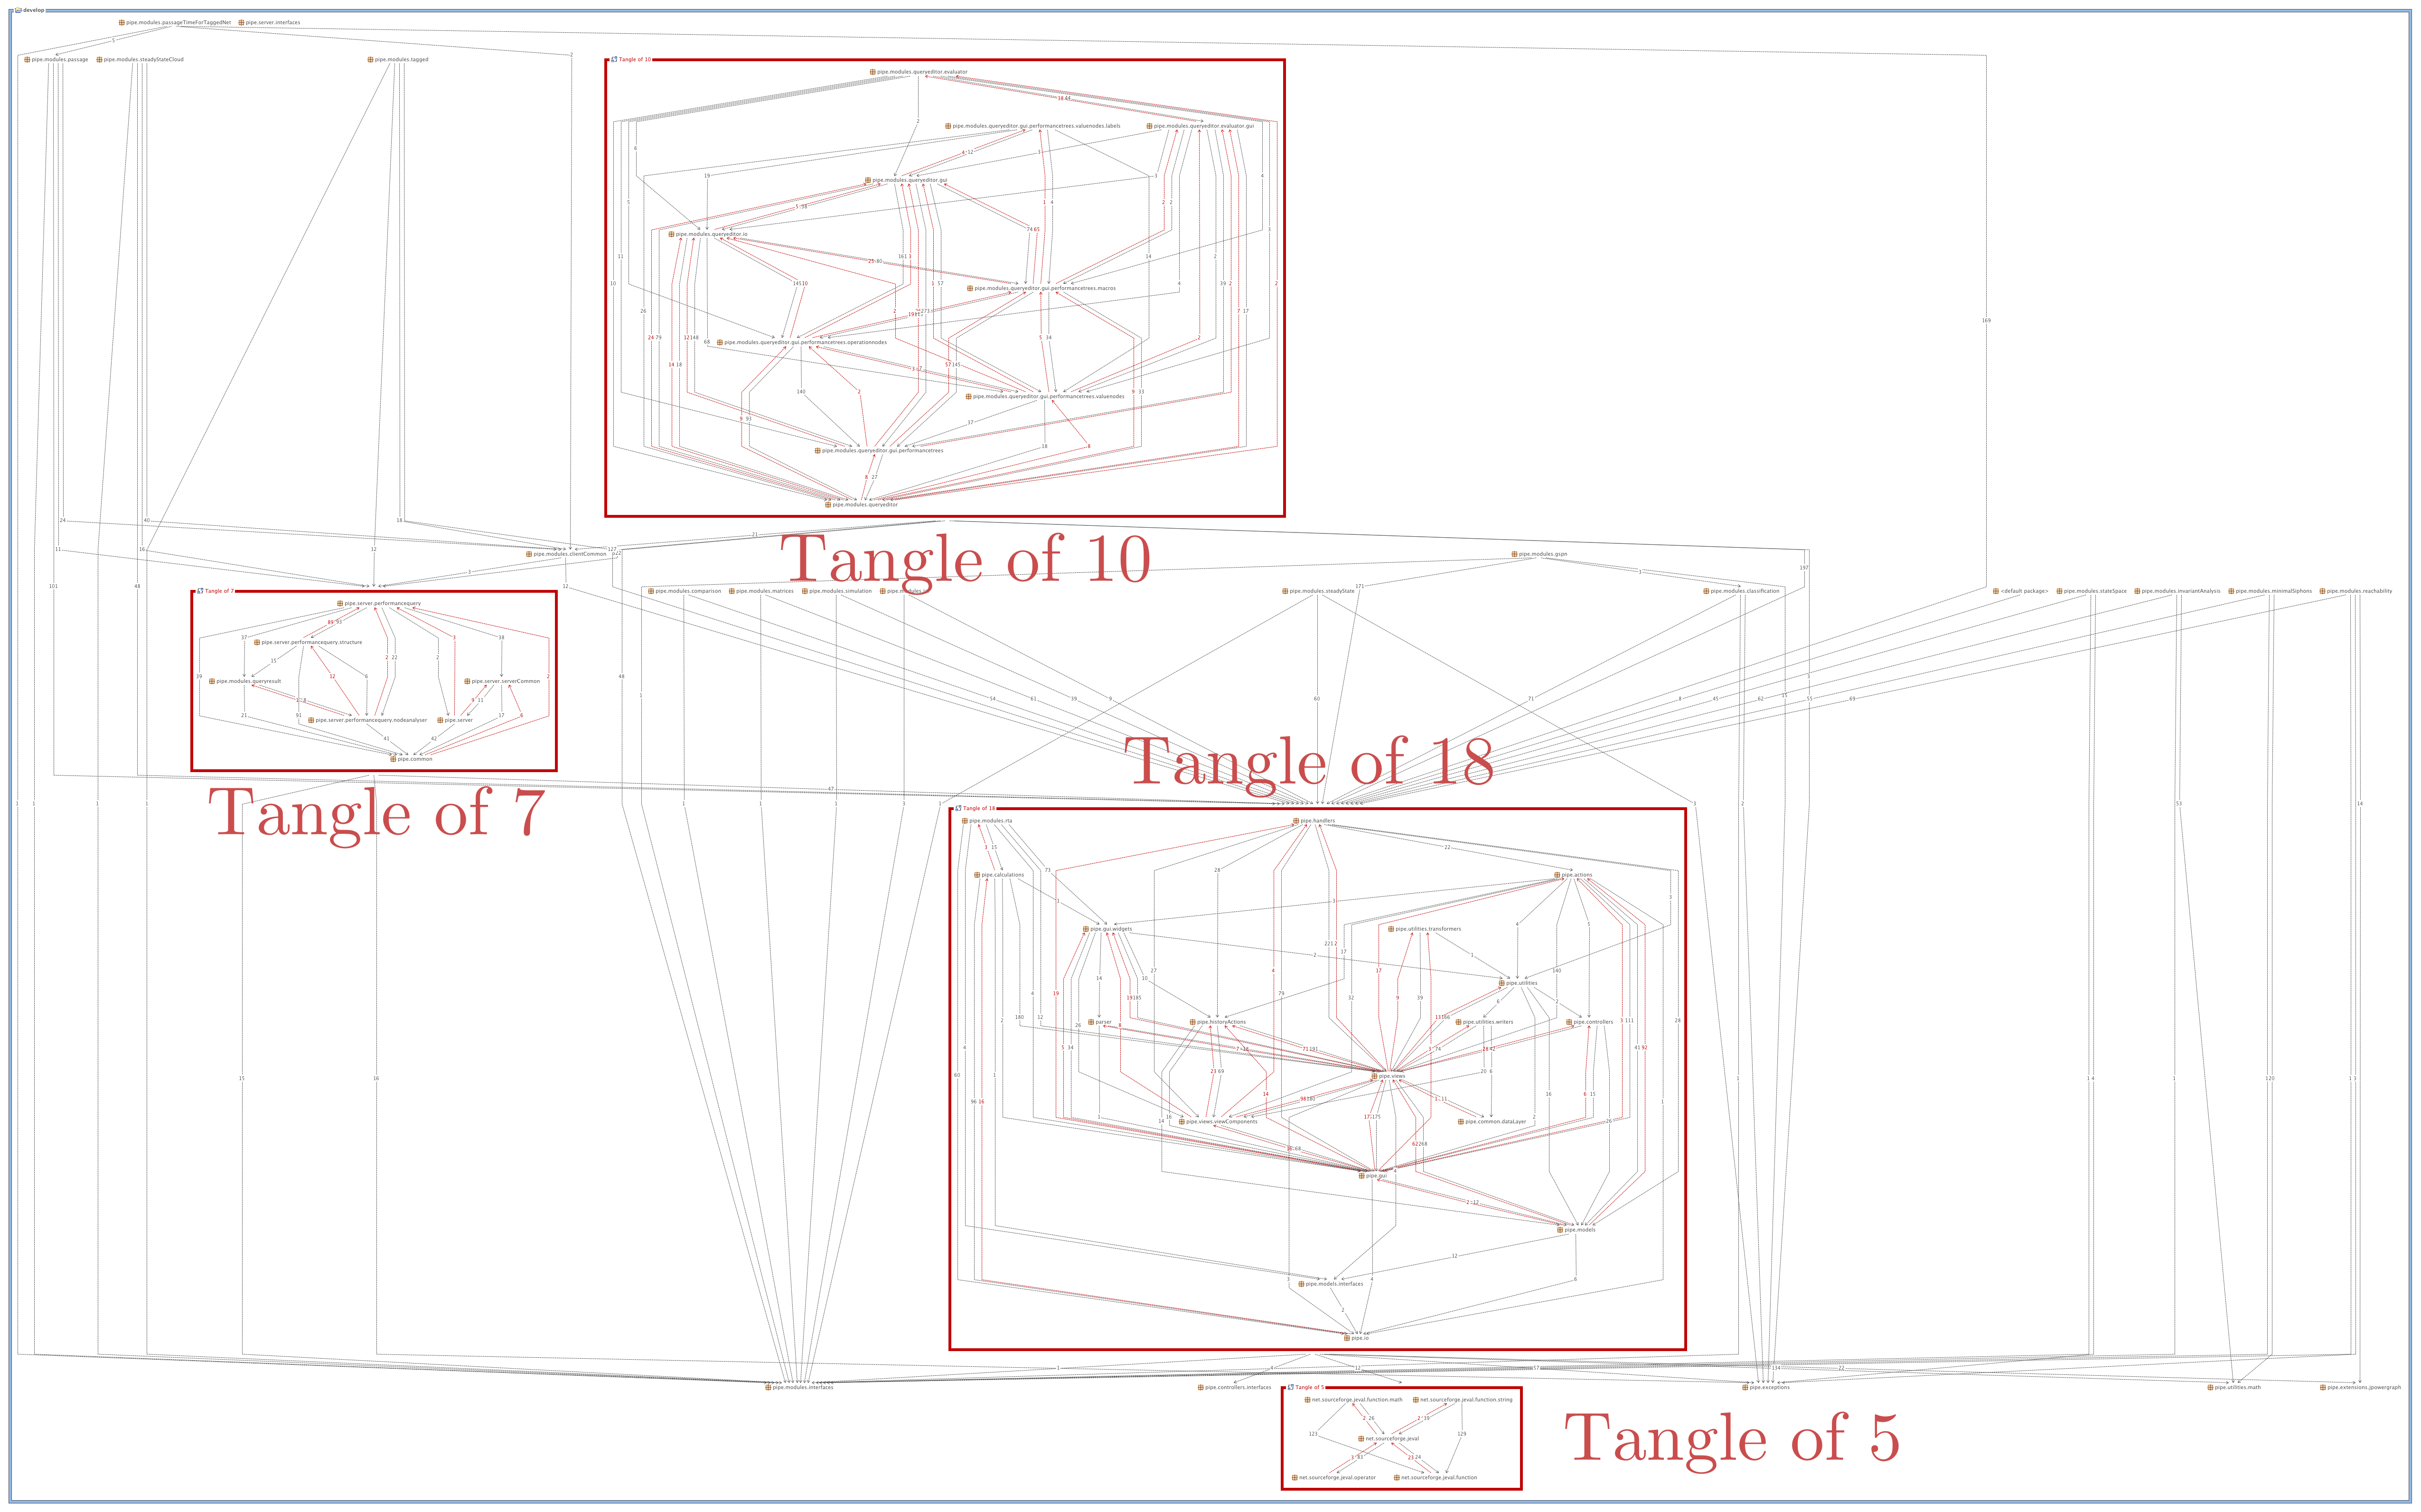
\includegraphics[width=0.85\textwidth]{eval/original_tangle_annotated.png} 
}
\subcaptionbox{The tangle graph for the PIPE repository housing the view code in PIPE 5 which contains the Swing GUI code. It contains only a single tangle of size 11. Unfortunately due to time constraints PIPE 5 uses much of the original PIPE 4 architecture which is why we were not able to reduce the tangle count further as many of the existing classes are tightly coupled. }{
    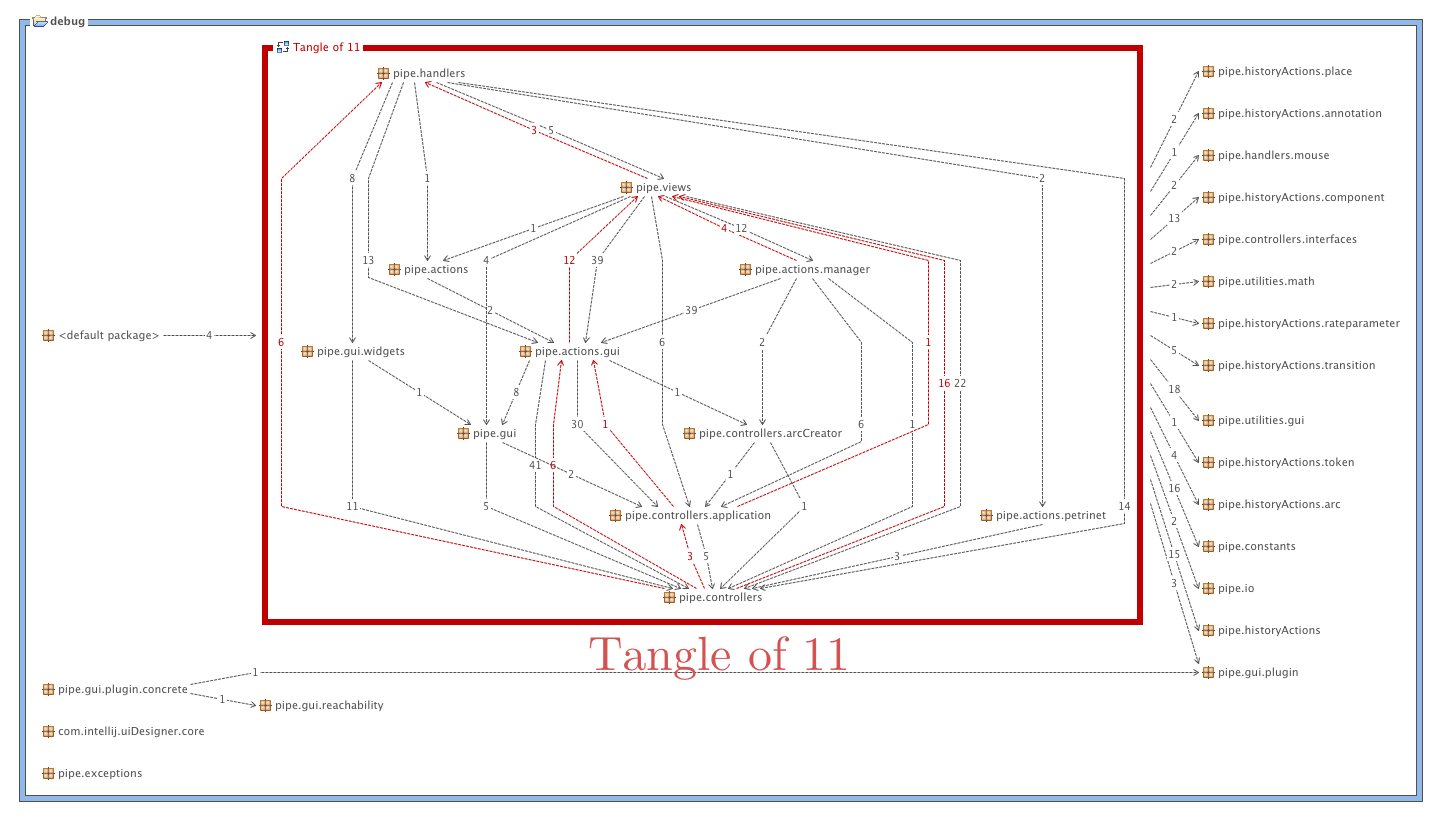
\includegraphics[width=0.85\textwidth]{eval/gui_tangle_annotated.png} 
}
% \caption{Tangle results}
\label{fig:tangle_results}
\end{center}
\end{figure}
\begin{figure}[tbp]
\begin{center}
\ContinuedFloat
\subcaptionbox{The new PIPE 5 tangle graph for the PIPECore repository reporting a single tangle of size 2. This tangle is between the functional expression parsers and the Petri net models. It has been kept because it improves the quality of the API by allowing Petri net components, namely transitions, to be able to evaluate their functional expressions without extra interaction from the user.}{
    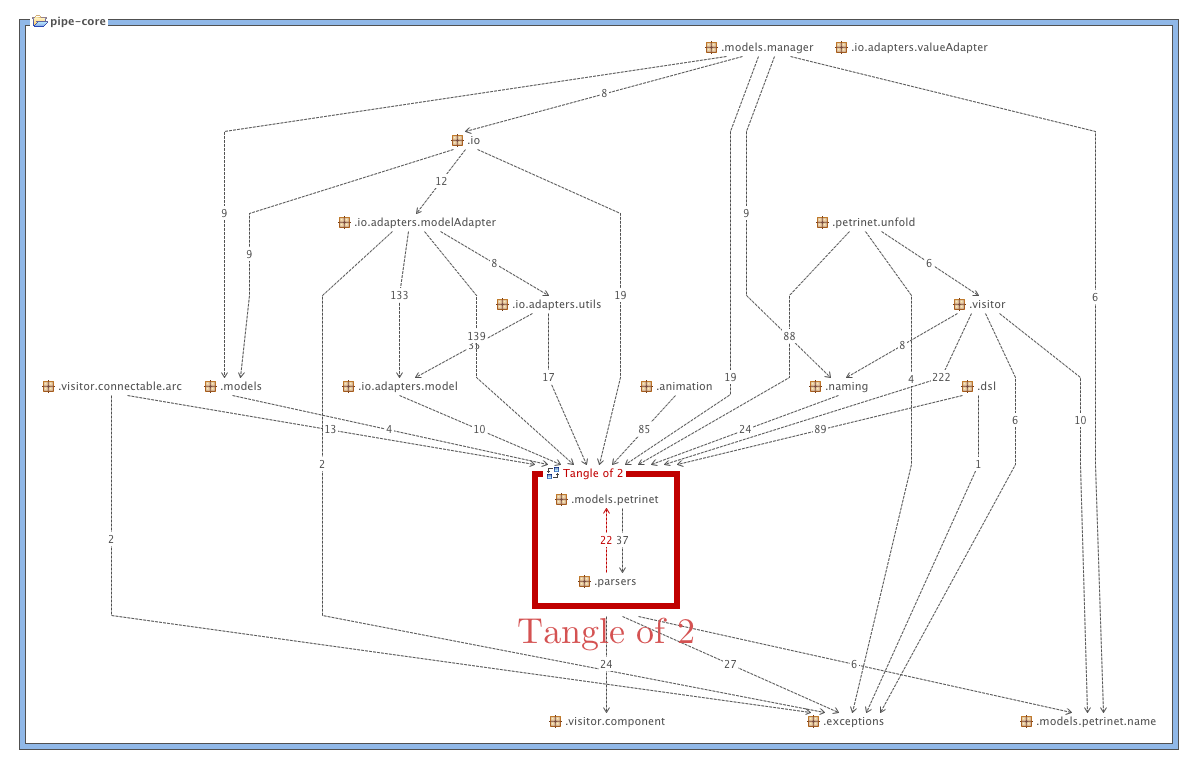
\includegraphics[width=0.85\textwidth]{eval/pipe_core_tangle_annotated.png} 
}
\subcaptionbox{The tangle graph for the new PIPEAnalysis repository containing the code for the steady state solver and the state space exploration. It reports 0 tangles.}{
    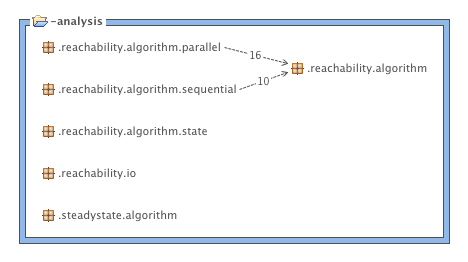
\includegraphics[scale=0.4]{eval/pipe_analysis_tangle.png} 
}
\hspace{5mm}
\subcaptionbox{The tangle graph for the new PIPEMarkovChain repository containing the classes which represent the underlying Markov chain of a Petri net and the explored sets data structure. It reports 0 tangles.}{
    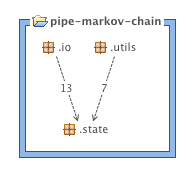
\includegraphics[scale=0.6]{eval/pipe_markov_chain_tangle.png} 
}
\caption{A comparison of the tangles in the PIPE 5 architecture against those in the PIPE 4 architecture. The tangle graphs clearly show a reduction from four tangles of size 18, 10, 7 and 5 down to only two tangles of size 11 and 2.}
\label{fig:tangle_results}
\end{center}
\end{figure}
\begin{table}[tb]
\small
\begin{center}
  \begin{tabular}{| l | c | c | c | c | c | c |}
    \hline
    Repository & Efficiency & Maintainability & Portability & Reliability & Usability & \textbf{Total} \\ 
    \hline
    PIPEMarkovChain & 0 & 0 & 0 & 0 & 0 & \textbf{0}\\ 
    \hline
    PIPEAnalysis & 0 & 0 & 0 & 0 & 0 & \textbf{0}\\    
    \hline
    PIPECore & 0 & 19 & 0 & 68 & 294 & \textbf{381}\\
    \hline
    PIPE & 13 & 77 & 0 & 426 & 40 & \textbf{556}\\
    \hline
    \textbf{Total} & \textbf{13} & \textbf{96} & \textbf{0} & \textbf{494} & \textbf{334} & {\color{red}\textbf{937}}\\
    \hline

  \end{tabular}
\caption{Break down of issues highlighted by the QAPlug analysis plug-in for Intellij for
each of the new PIPE 5 repositories. The total number of code quality issues for the entire project has been reduced from \num{12904} to \num{937}. Of these \num{937} issues \num{349} are due to auto-generated code via the ANTLR v4 plug-in.
Of the remaining issues in the PIPE codebase a total of \num{473} come from the \textit{`Magic Number Count'} metric and are due to layout and sizing settings for view components.
}
\label{tbl:pipe5_qaplug}
\end{center}
\end{table}
\begin{table}[tb]
\begin{center}
  \begin{tabular}{| c | c | c | c | c | }
  \hline
    Number of states & Number of transitions & PIPE 4 (s) & PIPE 5 (s) & Speedup \\
    \hline
    40 & 156 & 0.21 & 0.17 & 1.24\\
    \hline
    100 & 480 & 0.36 & 0.40 & 0.90\\
    \hline
    625 & 4000 & 25.12 & 1.35 & 18.61\\
    \hline
    1350 & 9450 & 83.67 & 1.75 & 47.81\\
    \hline
    4096 & 28672 & 728.02 & 3.82 & 190.58\\
    \hline
    11664 & 93312 & 2738.37 & 8.51 & 321.78\\
    \hline
  \end{tabular}
\caption{The time taken in seconds to generate the reachability graph in PIPE 4 compared with the new sequential algorithm in PIPE 5. For very small state spaces we can see that the times are comparable, but for moderate sized Petri nets PIPE 5 is more scalable.}
\label{tbl:pipe5_vs_pipe4_sequential}
\end{center}
\end{table}
\begin{figure}[ptb]
 \hspace*{\fill}%

\subcaptionbox{The raw times of the steady state exploration graph. The results gathered are for a sequential algorithm and for a parallel implementation with 100 states per thread running on 2, 4, and 8 virtual cores.} {
    \setfigname{}
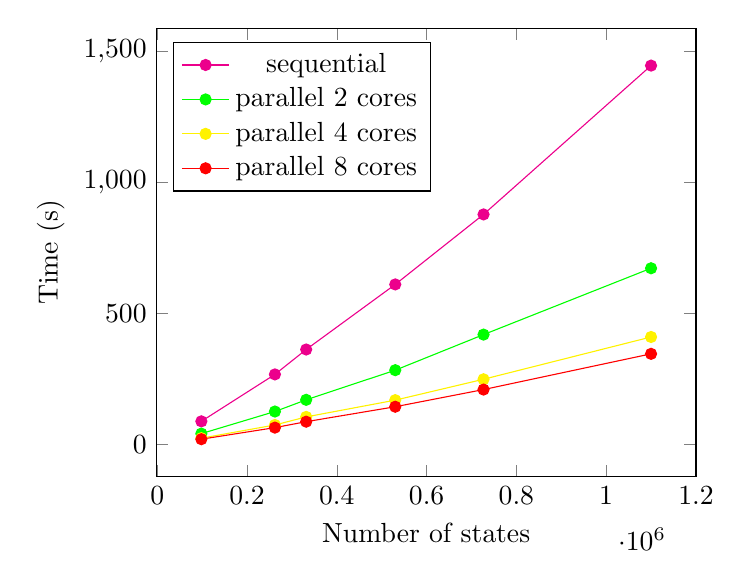
\begin{tikzpicture}
\definecolor{color0}{rgb}{0.75,0,0.75}

\begin{axis}[legend style={legend pos=north west},
ylabel={Time (s)},
xlabel={Number of states},
legend entries={{sequential},{parallel 2 cores},{parallel 4 cores},{parallel 8 cores}}
% scaled ticks=false
]

% Sequential
\addplot [magenta, mark=*, mark size=2pt]
coordinates {
(98279,     88.633369210) 
(262144,   267.658476596) 
(331776,   362.664597933) 
(530202,   610.926546563) 
(726836,   878.042343995) 
(1099999, 1445.821632163) 
};

% 2
\addplot [green, mark=*, mark size=2pt]
coordinates {
(98279,    41.786394435)
(262144,  126.064339906)
(331776,  170.664153825)
(530202,  283.808419361)
(726836,  419.506128369)
(1099999, 672.649284048)
};

% 4
\addplot [yellow, mark=*, mark size=2pt]
coordinates {
(98279,    24.373880968) 
(262144,   74.762257833) 
(331776,  105.559247500)
(530202,  169.459170682)
(726836,  249.133023117)
(1099999, 410.412285810)
};

% 8
\addplot [red, mark=*, mark size=2pt]
coordinates {
(98279,    20.521322935)  
(262144,   64.652309353)  
(331776,   87.323938113) 
(530202,  144.356493902) 
(726836,  209.819065630) 
(1099999, 346.097981548) 
};


\end{axis}
\end{tikzpicture}

}\hfill
\subcaptionbox{The relevant speedup gained over the sequential algorithm running our parallel algorithm with 100 states per thread and an increasing number of virtual cores. The graph shows that for each increase in the number of virtual cores we see a consistent speedup.} {
    \setfigname{}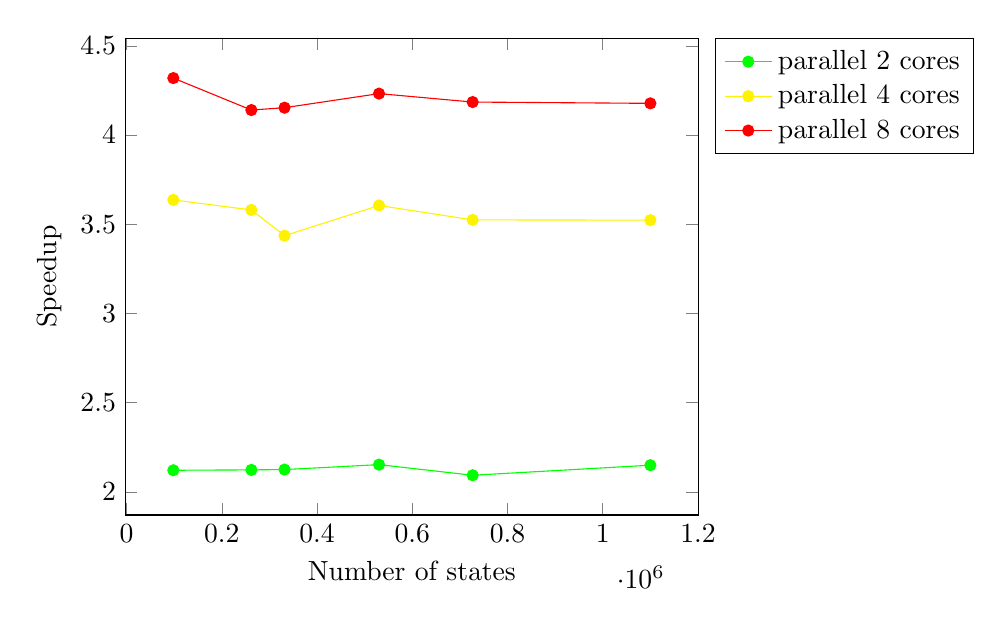
\begin{tikzpicture}
\definecolor{color0}{rgb}{0.75,0,0.75}

\begin{axis}[width=0.73\textwidth,
legend style={legend pos=outer north east},
ylabel={Speedup},
xlabel={Number of states},
legend entries={{parallel 2 cores},{parallel 4 cores},{parallel 8 cores}}
% scaled ticks=false
]

% 2
\addplot [green, mark=*, mark size=2pt]
coordinates {
(98279,   2.1211059343220406) % 99860326918 / 51611435904
(262144,  2.1231894506851012) % 304887660912 / 158793100442 
(331776,  2.1250191666193614) % 407267170985 / 208514610650
(530202,  2.152601913426362) % 709773626643 / 362338733157
(726836,  2.093038181369949) % 1023339231997 / 523542258224
(1099999, 2.149443501169068) % 1621045044327 / 845268409674
};

% 4
\addplot [yellow, mark=*, mark size=2pt]
coordinates {
(98279,   3.6364077319637786) % 99860326918 / 30575984607
(262144,  3.5801283208150485) % 304887660912 / 93863598681
(331776,  3.43564970878558) % 407267170985 / 127750195215
(530202,  3.605154823455611) % 709773626643 / 215606239138
(726836,  3.5243916402950974) % 1023339231997 / 318285464137
(1099999, 3.522851732641215) % 1621045044327 / 515475748470
};

% 8
\addplot [red, mark=*, mark size=2pt]
coordinates {
(98279,   4.319086517508672) % 99860326918 / 26825872545
(262144,  4.139967764099366) % 304887660912 / 82619391439
(331776,  4.153094853139814) % 407267170985 / 110556083237
(530202,  4.232068333397891) % 709773626643 / 189352805147
(726836,  4.184759575392262) % 1023339231997 / 282687963976
(1099999, 4.177492239903399) % 1621045044327 / 456685753436
};


\end{axis}
\end{tikzpicture}

}
\hspace*{\fill}%
\caption{A comparison between the run-times and relevant speedup of PIPE 5's sequential state space exploration and its parallel algorithm with 100 states per thread running on 2, 4 and 8 virtual cores on a 3.2GHz quad-core hyper-threaded 3rd generation i7 processor.}
\label{fig:scalability}
\end{figure}

